\documentclass[11pt, a4paper,twocolumn]{jarticle}
\usepackage[dvipdfmx]{graphicx}
\usepackage{listings,jlisting}

\begin{document}
%=============================================================
\section{Temprature dependence of the resistance($4^{th} day$)}

\subsection{Purpose}
金属抵抗の温度による変化を学ぶ.
\subsection{Procedure}
まず試料を四端子測定法の測定回路に接続する.次に熱電対と共に試料を固定し液体窒素の入った容器の中に沈めていく.
この時試料の温度は熱電対の起電力によって測定する.
今回使用した熱電対はクロメルーアルメル熱電対であり測定部分を氷水の容器に浸し基準を273Kにして測定する.
測定器の製作は図\ref{fig:29}のように組み立てる.

以上の手順でCu,NiCr,Wの低効率を測定していく.
測定は室温から77K程度まで5段階に分けて測定を行なった.
測定結果より抵抗値を最小二乗法で求めその温度依存性をグラフに示す.

\begin{figure}[htbp]
 \begin{center}
  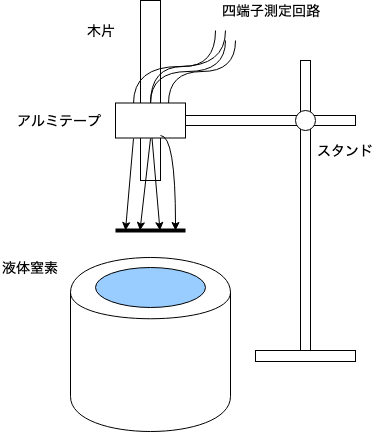
\includegraphics[width=0.8\linewidth]{fig29.png}
 \end{center}
 \caption{温度依存性の実験装置}
 \label{fig:29}
\end{figure}

\subsection{Result}
測定の結果温度と抵抗値の関係をプロットすると以下のようなグラフが得られた.

\begin{figure}[htbp]
 \begin{center}
  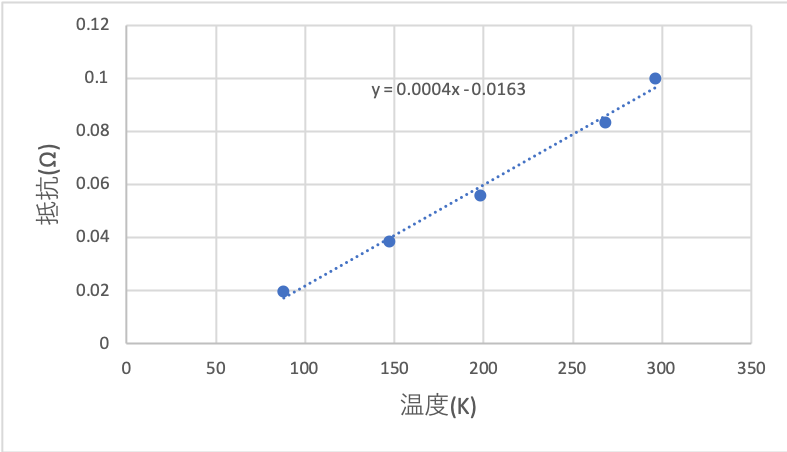
\includegraphics[width=0.8\linewidth]{fig30.png}
 \end{center}
 \caption{Wの温度依存}
 \label{fig:30}
\end{figure}

\begin{figure}[htbp]
 \begin{center}
  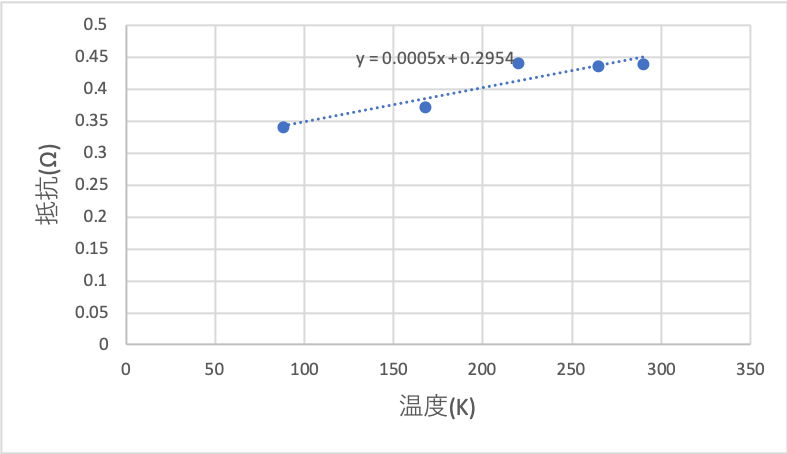
\includegraphics[width=0.8\linewidth]{fig31.png}
 \end{center}
 \caption{NiCrの温度依存}
 \label{fig:31}
\end{figure}

\begin{figure}[htbp]
 \begin{center}
  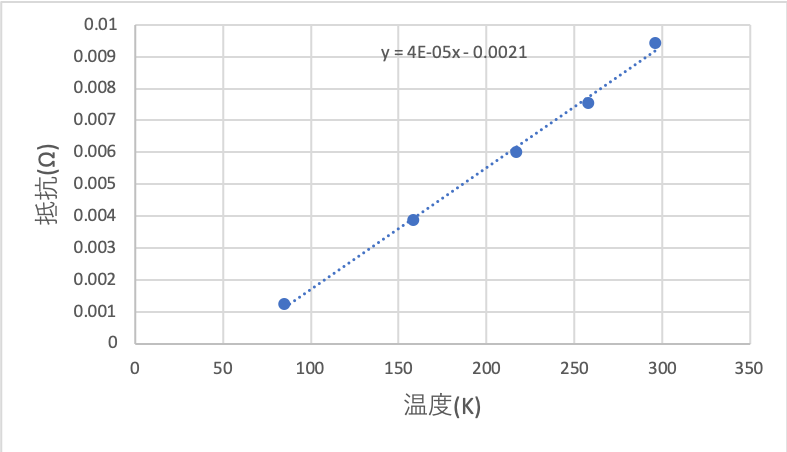
\includegraphics[width=0.8\linewidth]{fig32.png}
 \end{center}
 \caption{Cuの温度依存}
 \label{fig:32}
\end{figure}

\newpage


\subsection{Discussion}
実験結果より温度が低くなるにつれて抵抗率が小さくなった原因について考える.
まず前回の考察より金属中において電流の流れを阻害するものは熱振動する格子だと考えられることがわかった.したがって温度が下がるとその分熱運動により振動する格子の振動の激しさは穏やかになることが予想され結果として電流が格子と衝突する回数がすくなり流れる電流量が多くなり抵抗率が小さくなることが予想される.

%=============================================================
\newpage
\end{document}
